\PassOptionsToPackage{unicode=true}{hyperref} % options for packages loaded elsewhere
\PassOptionsToPackage{hyphens}{url}
%
\documentclass[]{article}
\usepackage{lmodern}
\usepackage{amssymb,amsmath}
\usepackage{ifxetex,ifluatex}
\usepackage{fixltx2e} % provides \textsubscript
\ifnum 0\ifxetex 1\fi\ifluatex 1\fi=0 % if pdftex
  \usepackage[T1]{fontenc}
  \usepackage[utf8]{inputenc}
  \usepackage{textcomp} % provides euro and other symbols
\else % if luatex or xelatex
  \usepackage{unicode-math}
  \defaultfontfeatures{Ligatures=TeX,Scale=MatchLowercase}
\fi
% use upquote if available, for straight quotes in verbatim environments
\IfFileExists{upquote.sty}{\usepackage{upquote}}{}
% use microtype if available
\IfFileExists{microtype.sty}{%
\usepackage[]{microtype}
\UseMicrotypeSet[protrusion]{basicmath} % disable protrusion for tt fonts
}{}
\IfFileExists{parskip.sty}{%
\usepackage{parskip}
}{% else
\setlength{\parindent}{0pt}
\setlength{\parskip}{6pt plus 2pt minus 1pt}
}
\usepackage{hyperref}
\hypersetup{
            pdftitle={Univariate time series examples - best practices},
            pdfauthor={Eric Ward},
            pdfborder={0 0 0},
            breaklinks=true}
\urlstyle{same}  % don't use monospace font for urls
\usepackage[margin=1in]{geometry}
\usepackage{color}
\usepackage{fancyvrb}
\newcommand{\VerbBar}{|}
\newcommand{\VERB}{\Verb[commandchars=\\\{\}]}
\DefineVerbatimEnvironment{Highlighting}{Verbatim}{commandchars=\\\{\}}
% Add ',fontsize=\small' for more characters per line
\usepackage{framed}
\definecolor{shadecolor}{RGB}{248,248,248}
\newenvironment{Shaded}{\begin{snugshade}}{\end{snugshade}}
\newcommand{\AlertTok}[1]{\textcolor[rgb]{0.94,0.16,0.16}{#1}}
\newcommand{\AnnotationTok}[1]{\textcolor[rgb]{0.56,0.35,0.01}{\textbf{\textit{#1}}}}
\newcommand{\AttributeTok}[1]{\textcolor[rgb]{0.77,0.63,0.00}{#1}}
\newcommand{\BaseNTok}[1]{\textcolor[rgb]{0.00,0.00,0.81}{#1}}
\newcommand{\BuiltInTok}[1]{#1}
\newcommand{\CharTok}[1]{\textcolor[rgb]{0.31,0.60,0.02}{#1}}
\newcommand{\CommentTok}[1]{\textcolor[rgb]{0.56,0.35,0.01}{\textit{#1}}}
\newcommand{\CommentVarTok}[1]{\textcolor[rgb]{0.56,0.35,0.01}{\textbf{\textit{#1}}}}
\newcommand{\ConstantTok}[1]{\textcolor[rgb]{0.00,0.00,0.00}{#1}}
\newcommand{\ControlFlowTok}[1]{\textcolor[rgb]{0.13,0.29,0.53}{\textbf{#1}}}
\newcommand{\DataTypeTok}[1]{\textcolor[rgb]{0.13,0.29,0.53}{#1}}
\newcommand{\DecValTok}[1]{\textcolor[rgb]{0.00,0.00,0.81}{#1}}
\newcommand{\DocumentationTok}[1]{\textcolor[rgb]{0.56,0.35,0.01}{\textbf{\textit{#1}}}}
\newcommand{\ErrorTok}[1]{\textcolor[rgb]{0.64,0.00,0.00}{\textbf{#1}}}
\newcommand{\ExtensionTok}[1]{#1}
\newcommand{\FloatTok}[1]{\textcolor[rgb]{0.00,0.00,0.81}{#1}}
\newcommand{\FunctionTok}[1]{\textcolor[rgb]{0.00,0.00,0.00}{#1}}
\newcommand{\ImportTok}[1]{#1}
\newcommand{\InformationTok}[1]{\textcolor[rgb]{0.56,0.35,0.01}{\textbf{\textit{#1}}}}
\newcommand{\KeywordTok}[1]{\textcolor[rgb]{0.13,0.29,0.53}{\textbf{#1}}}
\newcommand{\NormalTok}[1]{#1}
\newcommand{\OperatorTok}[1]{\textcolor[rgb]{0.81,0.36,0.00}{\textbf{#1}}}
\newcommand{\OtherTok}[1]{\textcolor[rgb]{0.56,0.35,0.01}{#1}}
\newcommand{\PreprocessorTok}[1]{\textcolor[rgb]{0.56,0.35,0.01}{\textit{#1}}}
\newcommand{\RegionMarkerTok}[1]{#1}
\newcommand{\SpecialCharTok}[1]{\textcolor[rgb]{0.00,0.00,0.00}{#1}}
\newcommand{\SpecialStringTok}[1]{\textcolor[rgb]{0.31,0.60,0.02}{#1}}
\newcommand{\StringTok}[1]{\textcolor[rgb]{0.31,0.60,0.02}{#1}}
\newcommand{\VariableTok}[1]{\textcolor[rgb]{0.00,0.00,0.00}{#1}}
\newcommand{\VerbatimStringTok}[1]{\textcolor[rgb]{0.31,0.60,0.02}{#1}}
\newcommand{\WarningTok}[1]{\textcolor[rgb]{0.56,0.35,0.01}{\textbf{\textit{#1}}}}
\usepackage{graphicx,grffile}
\makeatletter
\def\maxwidth{\ifdim\Gin@nat@width>\linewidth\linewidth\else\Gin@nat@width\fi}
\def\maxheight{\ifdim\Gin@nat@height>\textheight\textheight\else\Gin@nat@height\fi}
\makeatother
% Scale images if necessary, so that they will not overflow the page
% margins by default, and it is still possible to overwrite the defaults
% using explicit options in \includegraphics[width, height, ...]{}
\setkeys{Gin}{width=\maxwidth,height=\maxheight,keepaspectratio}
\setlength{\emergencystretch}{3em}  % prevent overfull lines
\providecommand{\tightlist}{%
  \setlength{\itemsep}{0pt}\setlength{\parskip}{0pt}}
\setcounter{secnumdepth}{0}
% Redefines (sub)paragraphs to behave more like sections
\ifx\paragraph\undefined\else
\let\oldparagraph\paragraph
\renewcommand{\paragraph}[1]{\oldparagraph{#1}\mbox{}}
\fi
\ifx\subparagraph\undefined\else
\let\oldsubparagraph\subparagraph
\renewcommand{\subparagraph}[1]{\oldsubparagraph{#1}\mbox{}}
\fi

% set default figure placement to htbp
\makeatletter
\def\fps@figure{htbp}
\makeatother


\title{Univariate time series examples - best practices}
\author{Eric Ward}
\date{2020-02-03}

\begin{document}
\maketitle

\hypertarget{data}{%
\subsection{Data}\label{data}}

I'm putting together a simple example with simulated data. This is
interesting because the observed response variable has a trend in
increasing variance. The mechanism is a time-varying but stationary
covariate, combined with a non-stationary coefficient between the
covariate and response.

\begin{Shaded}
\begin{Highlighting}[]
\KeywordTok{set.seed}\NormalTok{(}\DecValTok{123}\NormalTok{)}
\NormalTok{x =}\StringTok{ }\KeywordTok{scale}\NormalTok{(}\KeywordTok{cumsum}\NormalTok{(}\KeywordTok{rnorm}\NormalTok{(}\DecValTok{50}\NormalTok{)))}
\NormalTok{b =}\StringTok{ }\KeywordTok{cumsum}\NormalTok{(}\KeywordTok{rnorm}\NormalTok{(}\DataTypeTok{n=}\KeywordTok{length}\NormalTok{(x),}\DecValTok{0}\NormalTok{,}\FloatTok{0.02}\NormalTok{))}
\NormalTok{y =}\StringTok{ }\KeywordTok{rnorm}\NormalTok{(}\DecValTok{3}\OperatorTok{+}\NormalTok{x}\OperatorTok{*}\NormalTok{b, }\FloatTok{0.1}\NormalTok{)}
\NormalTok{dat =}\StringTok{ }\KeywordTok{data.frame}\NormalTok{(}\DataTypeTok{time=}\KeywordTok{seq}\NormalTok{(}\DecValTok{1}\NormalTok{,}\KeywordTok{length}\NormalTok{(x)),}\DataTypeTok{x=}\NormalTok{x,}\DataTypeTok{y=}\NormalTok{y,}\DataTypeTok{b=}\NormalTok{b)}

\NormalTok{g1 =}\StringTok{ }\NormalTok{ggplot2}\OperatorTok{::}\KeywordTok{ggplot}\NormalTok{(dat,}\KeywordTok{aes}\NormalTok{(time,x)) }\OperatorTok{+}\StringTok{ }\KeywordTok{geom_point}\NormalTok{() }\OperatorTok{+}\StringTok{ }
\StringTok{  }\KeywordTok{xlab}\NormalTok{(}\StringTok{"Time"}\NormalTok{) }\OperatorTok{+}\StringTok{ }\KeywordTok{ylab}\NormalTok{(}\StringTok{"x covariate"}\NormalTok{)}
\NormalTok{g2 =}\StringTok{ }\NormalTok{ggplot2}\OperatorTok{::}\KeywordTok{ggplot}\NormalTok{(dat,}\KeywordTok{aes}\NormalTok{(time,b)) }\OperatorTok{+}\StringTok{ }\KeywordTok{geom_point}\NormalTok{() }\OperatorTok{+}\StringTok{ }
\StringTok{  }\KeywordTok{xlab}\NormalTok{(}\StringTok{"Time"}\NormalTok{) }\OperatorTok{+}\StringTok{ }\KeywordTok{ylab}\NormalTok{(}\StringTok{"b coefficient"}\NormalTok{)}
\NormalTok{g3 =}\StringTok{ }\NormalTok{ggplot2}\OperatorTok{::}\KeywordTok{ggplot}\NormalTok{(dat,}\KeywordTok{aes}\NormalTok{(time,y)) }\OperatorTok{+}\StringTok{ }\KeywordTok{geom_point}\NormalTok{() }\OperatorTok{+}\StringTok{ }
\StringTok{  }\KeywordTok{xlab}\NormalTok{(}\StringTok{"Time"}\NormalTok{) }\OperatorTok{+}\StringTok{ }\KeywordTok{ylab}\NormalTok{(}\StringTok{"Data (y)"}\NormalTok{)}
\NormalTok{gridExtra}\OperatorTok{::}\KeywordTok{grid.arrange}\NormalTok{(g1,g2,g3,}\DataTypeTok{nrow=}\DecValTok{3}\NormalTok{)}
\end{Highlighting}
\end{Shaded}

\begin{figure}
\centering
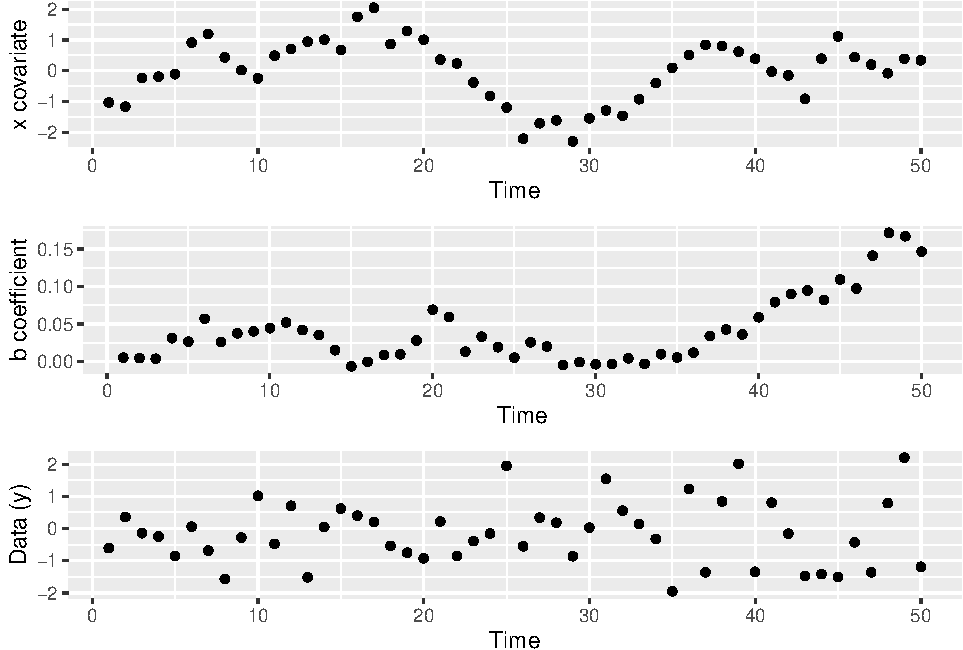
\includegraphics{univariate-time-series-examples_files/figure-latex/unnamed-chunk-1-1.pdf}
\caption{Simulated data and covariate. The predicted data at each time
step is a linear function of the covariate, y(t) = b0 + b1(t) * x(t)}
\end{figure}

\hypertarget{linear-regression-and-time-series-models}{%
\subsubsection{Linear regression and time series
models}\label{linear-regression-and-time-series-models}}

\begin{Shaded}
\begin{Highlighting}[]
\CommentTok{# start with linear regression, no breakpoint in year 30}
\NormalTok{fit <-}\StringTok{ }\KeywordTok{brm}\NormalTok{(y }\OperatorTok{~}\StringTok{ }\NormalTok{x }\OperatorTok{*}\StringTok{ }\NormalTok{b,}\DataTypeTok{data=}\NormalTok{dat)}
\NormalTok{dat}\OperatorTok{$}\NormalTok{breaks =}\StringTok{ }\KeywordTok{c}\NormalTok{(}\KeywordTok{rep}\NormalTok{(}\StringTok{"pre"}\NormalTok{,}\DecValTok{30}\NormalTok{),}\KeywordTok{rep}\NormalTok{(}\StringTok{"post"}\NormalTok{,}\DecValTok{20}\NormalTok{))}
\NormalTok{dat}\OperatorTok{$}\NormalTok{pred =}\StringTok{ }\KeywordTok{predict}\NormalTok{(fit,}\DataTypeTok{newdata=}\NormalTok{dat)[,}\StringTok{"Estimate"}\NormalTok{]}
\NormalTok{dat}\OperatorTok{$}\NormalTok{model =}\StringTok{ "lm"}
\NormalTok{results =}\StringTok{ }\NormalTok{dat}
  
\CommentTok{# next linear regression, fixed breakpoint in year 30}
\NormalTok{fit =}\StringTok{ }\KeywordTok{brm}\NormalTok{(y }\OperatorTok{~}\StringTok{ }\NormalTok{x }\OperatorTok{*}\StringTok{ }\NormalTok{b }\OperatorTok{+}\StringTok{ }\NormalTok{b}\OperatorTok{*}\NormalTok{breaks,}\DataTypeTok{data=}\NormalTok{dat)}
\NormalTok{dat}\OperatorTok{$}\NormalTok{pred =}\StringTok{ }\KeywordTok{predict}\NormalTok{(fit,}\DataTypeTok{newdata=}\NormalTok{dat)[,}\StringTok{"Estimate"}\NormalTok{]}
\NormalTok{dat}\OperatorTok{$}\NormalTok{model =}\StringTok{ "lm - fixed breakpoint"}
\NormalTok{results =}\StringTok{ }\KeywordTok{rbind}\NormalTok{(results,dat)}

\CommentTok{# add linear time series model, with AR(1) and MA(1) components}
\NormalTok{fit =}\StringTok{ }\KeywordTok{arima}\NormalTok{(dat}\OperatorTok{$}\NormalTok{y, }\DataTypeTok{xreg=}\NormalTok{dat}\OperatorTok{$}\NormalTok{x, }\DataTypeTok{order =} \KeywordTok{c}\NormalTok{(}\DecValTok{1}\NormalTok{,}\DecValTok{0}\NormalTok{,}\DecValTok{1}\NormalTok{))}
\NormalTok{dat}\OperatorTok{$}\NormalTok{pred =}\StringTok{ }\KeywordTok{fitted}\NormalTok{(fit)}
\NormalTok{dat}\OperatorTok{$}\NormalTok{model =}\StringTok{ "ARIMA (1,0,1)"}
\NormalTok{results =}\StringTok{ }\KeywordTok{rbind}\NormalTok{(results,dat)}
\end{Highlighting}
\end{Shaded}

\hypertarget{dlm-models}{%
\subsubsection{DLM models}\label{dlm-models}}

Dynamic linear models are state space models, and can have random walks
in intercept, slope or both. Either are considered process variation.

\begin{Shaded}
\begin{Highlighting}[]
\CommentTok{# Random walk on slope here:}
\NormalTok{fit =}\StringTok{ }\KeywordTok{fit_stan}\NormalTok{(}\DataTypeTok{y =}\NormalTok{ dat}\OperatorTok{$}\NormalTok{y, }\DataTypeTok{x =}\NormalTok{ dat}\OperatorTok{$}\NormalTok{x, }\DataTypeTok{model_name=}\StringTok{"dlm-slope"}\NormalTok{)}
\NormalTok{dat}\OperatorTok{$}\NormalTok{pred =}\StringTok{ }\KeywordTok{apply}\NormalTok{(rstan}\OperatorTok{::}\KeywordTok{extract}\NormalTok{(fit)}\OperatorTok{$}\NormalTok{pred,}\DecValTok{2}\NormalTok{,mean)}
\NormalTok{dat}\OperatorTok{$}\NormalTok{model =}\StringTok{ "dlm-slope"}
\NormalTok{results =}\StringTok{ }\KeywordTok{rbind}\NormalTok{(results,dat)}

\CommentTok{# time varying slope, constant intercept}
\NormalTok{fit =}\StringTok{ }\KeywordTok{fit_stan}\NormalTok{(}\DataTypeTok{y =}\NormalTok{ dat}\OperatorTok{$}\NormalTok{y, }\DataTypeTok{x =}\NormalTok{ dat}\OperatorTok{$}\NormalTok{x, }\DataTypeTok{model_name=}\StringTok{"dlm-intercept"}\NormalTok{)}
\NormalTok{dat}\OperatorTok{$}\NormalTok{pred =}\StringTok{ }\KeywordTok{apply}\NormalTok{(rstan}\OperatorTok{::}\KeywordTok{extract}\NormalTok{(fit)}\OperatorTok{$}\NormalTok{pred,}\DecValTok{2}\NormalTok{,mean)}
\NormalTok{dat}\OperatorTok{$}\NormalTok{model =}\StringTok{ "dlm-intercept"}
\NormalTok{results =}\StringTok{ }\KeywordTok{rbind}\NormalTok{(results,dat)}

\CommentTok{# time varying slope and intercept. some issues with identifiability}
\NormalTok{fit =}\StringTok{ }\KeywordTok{fit_stan}\NormalTok{(}\DataTypeTok{y =}\NormalTok{ dat}\OperatorTok{$}\NormalTok{y, }\DataTypeTok{x =} \KeywordTok{model.matrix}\NormalTok{(}\KeywordTok{lm}\NormalTok{(dat}\OperatorTok{$}\NormalTok{y}\OperatorTok{~}\NormalTok{dat}\OperatorTok{$}\NormalTok{x)), }\DataTypeTok{model_name=}\StringTok{"dlm"}\NormalTok{)}
\NormalTok{dat}\OperatorTok{$}\NormalTok{pred =}\StringTok{ }\KeywordTok{apply}\NormalTok{(rstan}\OperatorTok{::}\KeywordTok{extract}\NormalTok{(fit)}\OperatorTok{$}\NormalTok{pred,}\DecValTok{2}\NormalTok{,mean)}
\NormalTok{dat}\OperatorTok{$}\NormalTok{model =}\StringTok{ "dlm-both"}
\NormalTok{results =}\StringTok{ }\KeywordTok{rbind}\NormalTok{(results,dat)}
\end{Highlighting}
\end{Shaded}

\hypertarget{genaralized-additive-models}{%
\subsubsection{Genaralized Additive
Models}\label{genaralized-additive-models}}

\begin{Shaded}
\begin{Highlighting}[]
\CommentTok{# GAM - simple}
\NormalTok{fit =}\StringTok{ }\KeywordTok{gam}\NormalTok{(y }\OperatorTok{~}\StringTok{ }\KeywordTok{s}\NormalTok{(x), }\DataTypeTok{data=}\NormalTok{dat)}
\NormalTok{dat}\OperatorTok{$}\NormalTok{pred =}\StringTok{ }\NormalTok{fit}\OperatorTok{$}\NormalTok{fitted.values}
\NormalTok{dat}\OperatorTok{$}\NormalTok{model =}\StringTok{ "gam s(x)"}
\NormalTok{results =}\StringTok{ }\KeywordTok{rbind}\NormalTok{(results,dat)}

\CommentTok{# GAM, AR errors}
\NormalTok{fit =}\StringTok{ }\KeywordTok{gamm}\NormalTok{(y }\OperatorTok{~}\StringTok{ }\KeywordTok{s}\NormalTok{(x),}\DataTypeTok{correlation =} \KeywordTok{corARMA}\NormalTok{(}\DataTypeTok{p=}\DecValTok{1}\NormalTok{), }\DataTypeTok{data=}\NormalTok{dat)}
\NormalTok{dat}\OperatorTok{$}\NormalTok{pred =}\StringTok{ }\NormalTok{fit}\OperatorTok{$}\NormalTok{gam}\OperatorTok{$}\NormalTok{fitted.values}
\NormalTok{dat}\OperatorTok{$}\NormalTok{model =}\StringTok{ "gam s(x) & MA"}
\NormalTok{results =}\StringTok{ }\KeywordTok{rbind}\NormalTok{(results,dat)}

\CommentTok{# GAM, interaction between x and time}
\NormalTok{fit =}\StringTok{ }\KeywordTok{gam}\NormalTok{(y }\OperatorTok{~}\StringTok{ }\KeywordTok{s}\NormalTok{(x) }\OperatorTok{+}\StringTok{ }\KeywordTok{s}\NormalTok{(time) }\OperatorTok{+}\StringTok{ }\KeywordTok{ti}\NormalTok{(x,time), }\DataTypeTok{data=}\NormalTok{dat)}
\NormalTok{dat}\OperatorTok{$}\NormalTok{pred =}\StringTok{ }\NormalTok{fit}\OperatorTok{$}\NormalTok{fitted.values}
\NormalTok{dat}\OperatorTok{$}\NormalTok{model =}\StringTok{ "gam te(x,time)"}
\NormalTok{results =}\StringTok{ }\KeywordTok{rbind}\NormalTok{(results,dat)}

\CommentTok{# GAM with time-varying coefficient}
\NormalTok{fit =}\StringTok{ }\KeywordTok{gam}\NormalTok{(y }\OperatorTok{~}\StringTok{ }\KeywordTok{s}\NormalTok{(time,}\DataTypeTok{by=}\NormalTok{x), }\DataTypeTok{data=}\NormalTok{dat)}
\NormalTok{dat}\OperatorTok{$}\NormalTok{pred =}\StringTok{ }\NormalTok{fit}\OperatorTok{$}\NormalTok{fitted.values}
\NormalTok{dat}\OperatorTok{$}\NormalTok{model =}\StringTok{ "gam time varying"}
\NormalTok{results =}\StringTok{ }\KeywordTok{rbind}\NormalTok{(results,dat)}
\end{Highlighting}
\end{Shaded}

\hypertarget{hidden-markov-models-hmms}{%
\subsubsection{Hidden Markov Models
(HMMs)}\label{hidden-markov-models-hmms}}

Hidden Markov Models or discrete state switching models have an
underlying latent state that each time point can be assigned to, and
this state evolves as a Markov process with transition matrix Gamma (m x
m). Though we could have \textgreater{} 2 states in the model,
estimation becomes more difficult, so we'll restrict this to the 2-state
model for now. Each state in the model might have a different mean or
variance. Two examples are below, (1) each state is allowed to have a
separate regression coefficient, and (2) each state is allowed to have
separate regression coefficients and residual errors.

\begin{Shaded}
\begin{Highlighting}[]
\CommentTok{# Hidden markov model / 2 regime switching for b 1 coefficient}
\NormalTok{jagsscript =}\StringTok{ }\KeywordTok{cat}\NormalTok{(}\StringTok{"}
\StringTok{model \{ }
\StringTok{  # priors for intercept}
\StringTok{  B0 ~ dnorm(0,1);}
\StringTok{  # priors for regression coefficient}
\StringTok{  for(i in 1:2) \{}
\StringTok{    B1[i] ~ dnorm(0,1);}
\StringTok{  \}}
\StringTok{  # prior for obs Error}
\StringTok{  obsTau ~ dgamma(0.001,0.001);}
\StringTok{  obsSigma <- 1/sqrt(obsTau);}

\StringTok{  # markov switching}
\StringTok{  alpha[1] <- 1;}
\StringTok{  alpha[2] <- 1;}
\StringTok{  p[1:2] ~ ddirch(alpha[1:2]);}
\StringTok{  Gamma[1,1:2] ~ ddirch(alpha[1:2]);}
\StringTok{  Gamma[2,1:2] ~ ddirch(alpha[1:2]);}
\StringTok{  z[1] ~ dcat(p[1:2]);}
\StringTok{  for(n in 2:nT) \{}
\StringTok{    z[n] ~ dcat(Gamma[z[n-1],]);}
\StringTok{  \}}

\StringTok{  # evaluate the likelihood}
\StringTok{  for(n in 1:nT) \{}
\StringTok{  pred[n] <- B0 + B1[z[n]]*x[n];}
\StringTok{  y[n] ~ dnorm(pred[n],obsTau);}
\StringTok{  \}    }
\StringTok{  \}  "}\NormalTok{,}\DataTypeTok{file=}\StringTok{"jags_switching.txt"}\NormalTok{)}

\NormalTok{jags.data =}\StringTok{ }\KeywordTok{list}\NormalTok{(}\StringTok{"y"}\NormalTok{=dat}\OperatorTok{$}\NormalTok{y,}\StringTok{"x"}\NormalTok{=dat}\OperatorTok{$}\NormalTok{x,}\StringTok{"nT"}\NormalTok{=}\KeywordTok{nrow}\NormalTok{(dat))}
\NormalTok{jags.params=}\KeywordTok{c}\NormalTok{(}\StringTok{"B0"}\NormalTok{,}\StringTok{"B1"}\NormalTok{,}\StringTok{"pred"}\NormalTok{,}\StringTok{"z"}\NormalTok{)}
\NormalTok{model.loc=(}\StringTok{"jags_switching.txt"}\NormalTok{)}

\NormalTok{jags.model =}\StringTok{ }\KeywordTok{jags}\NormalTok{(jags.data, }\DataTypeTok{inits =} \OtherTok{NULL}\NormalTok{, }
  \DataTypeTok{parameters.to.save=}\NormalTok{ jags.params, }
  \DataTypeTok{model.file=}\NormalTok{model.loc, }
  \DataTypeTok{n.chains =} \DecValTok{3}\NormalTok{, }
  \DataTypeTok{n.burnin =} \DecValTok{20000}\NormalTok{, }
  \DataTypeTok{n.thin =} \DecValTok{1}\NormalTok{, }
  \DataTypeTok{n.iter =} \DecValTok{30000}\NormalTok{)  }
\KeywordTok{attach.jags}\NormalTok{(jags.model, }\DataTypeTok{overwrite=}\OtherTok{TRUE}\NormalTok{)}
\NormalTok{dat}\OperatorTok{$}\NormalTok{pred =}\StringTok{ }\KeywordTok{apply}\NormalTok{(pred,}\DecValTok{2}\NormalTok{,mean)}
\NormalTok{dat}\OperatorTok{$}\NormalTok{model =}\StringTok{ "HMM - b"}
\NormalTok{results =}\StringTok{ }\KeywordTok{rbind}\NormalTok{(results,dat)}

\CommentTok{# Hidden markov model / 2 regime switching for b 1 coefficient}
\NormalTok{jagsscript =}\StringTok{ }\KeywordTok{cat}\NormalTok{(}\StringTok{"}
\StringTok{  model \{   }
\StringTok{  # priors for intercept}
\StringTok{  B0 ~ dnorm(0,1);}
\StringTok{  # priors for regression coefficient}
\StringTok{  for(i in 1:2) \{}
\StringTok{  B1[i] ~ dnorm(0,1);}
\StringTok{  \}}
\StringTok{  # prior for obs Error}
\StringTok{  obsTau[1] ~ dgamma(0.001,0.001);}
\StringTok{  obsSigma[1] <- 1/sqrt(obsTau[1]);}
\StringTok{  obsTau[2] ~ dgamma(0.001,0.001);}
\StringTok{  obsSigma[2] <- 1/sqrt(obsTau[2]);}

\StringTok{  # markov switching}
\StringTok{  alpha[1] <- 1;}
\StringTok{  alpha[2] <- 1;}
\StringTok{  p[1:2] ~ ddirch(alpha[1:2]);}
\StringTok{  Gamma[1,1:2] ~ ddirch(alpha[1:2]);}
\StringTok{  Gamma[2,1:2] ~ ddirch(alpha[1:2]);}
\StringTok{  z[1] ~ dcat(p[1:2]);}
\StringTok{  for(n in 2:nT) \{}
\StringTok{  z[n] ~ dcat(Gamma[z[n-1],]);}
\StringTok{  \}}
\StringTok{  }
\StringTok{  # evaluate the likelihood}
\StringTok{  for(n in 1:nT) \{}
\StringTok{  pred[n] <- B0 + B1[z[n]]*x[n];}
\StringTok{  y[n] ~ dnorm(pred[n],obsTau[z[n]]);}
\StringTok{  \}    }
\StringTok{  \}  "}\NormalTok{,}\DataTypeTok{file=}\StringTok{"jags_switching_var.txt"}\NormalTok{)}

\NormalTok{jags.data =}\StringTok{ }\KeywordTok{list}\NormalTok{(}\StringTok{"y"}\NormalTok{=dat}\OperatorTok{$}\NormalTok{y,}\StringTok{"x"}\NormalTok{=dat}\OperatorTok{$}\NormalTok{x,}\StringTok{"nT"}\NormalTok{=}\KeywordTok{nrow}\NormalTok{(dat))}
\NormalTok{jags.params=}\KeywordTok{c}\NormalTok{(}\StringTok{"B0"}\NormalTok{,}\StringTok{"B1"}\NormalTok{,}\StringTok{"pred"}\NormalTok{,}\StringTok{"z"}\NormalTok{)}
\NormalTok{model.loc=(}\StringTok{"jags_switching_var.txt"}\NormalTok{)}

\NormalTok{jags.model =}\StringTok{ }\KeywordTok{jags}\NormalTok{(jags.data, }\DataTypeTok{inits =} \OtherTok{NULL}\NormalTok{, }
  \DataTypeTok{parameters.to.save=}\NormalTok{ jags.params, }
  \DataTypeTok{model.file=}\NormalTok{model.loc, }
  \DataTypeTok{n.chains =} \DecValTok{3}\NormalTok{, }
  \DataTypeTok{n.burnin =} \DecValTok{20000}\NormalTok{, }
  \DataTypeTok{n.thin =} \DecValTok{1}\NormalTok{, }
  \DataTypeTok{n.iter =} \DecValTok{30000}\NormalTok{)  }
\KeywordTok{attach.jags}\NormalTok{(jags.model, }\DataTypeTok{overwrite=}\OtherTok{TRUE}\NormalTok{)}
\NormalTok{dat}\OperatorTok{$}\NormalTok{pred =}\StringTok{ }\KeywordTok{apply}\NormalTok{(pred,}\DecValTok{2}\NormalTok{,mean)}
\NormalTok{dat}\OperatorTok{$}\NormalTok{model =}\StringTok{ "HMM - b & var"}
\NormalTok{results =}\StringTok{ }\KeywordTok{rbind}\NormalTok{(results,dat)}
\end{Highlighting}
\end{Shaded}

\hypertarget{plotting-results}{%
\subsection{Plotting Results}\label{plotting-results}}

\begin{Shaded}
\begin{Highlighting}[]
\CommentTok{# reorder levels to be ordered in the order they were fit}
\NormalTok{results}\OperatorTok{$}\NormalTok{model =}\StringTok{ }\KeywordTok{factor}\NormalTok{(results}\OperatorTok{$}\NormalTok{model,}
  \DataTypeTok{levels =} \KeywordTok{unique}\NormalTok{(results}\OperatorTok{$}\NormalTok{model))}
\end{Highlighting}
\end{Shaded}

\begin{Shaded}
\begin{Highlighting}[]
\CommentTok{# plot residuals across modeling approaches}
\KeywordTok{ggplot}\NormalTok{(results, }\KeywordTok{aes}\NormalTok{(time,y}\OperatorTok{-}\NormalTok{pred)) }\OperatorTok{+}\StringTok{ }\KeywordTok{geom_point}\NormalTok{() }\OperatorTok{+}\StringTok{ }
\StringTok{  }\KeywordTok{facet_wrap}\NormalTok{(}\OperatorTok{~}\NormalTok{model) }\OperatorTok{+}\StringTok{ }\KeywordTok{xlab}\NormalTok{(}\StringTok{"Time"}\NormalTok{) }\OperatorTok{+}\StringTok{ }\KeywordTok{ylab}\NormalTok{(}\StringTok{"Y - E[Y]"}\NormalTok{)}
\end{Highlighting}
\end{Shaded}

\begin{figure}
\centering
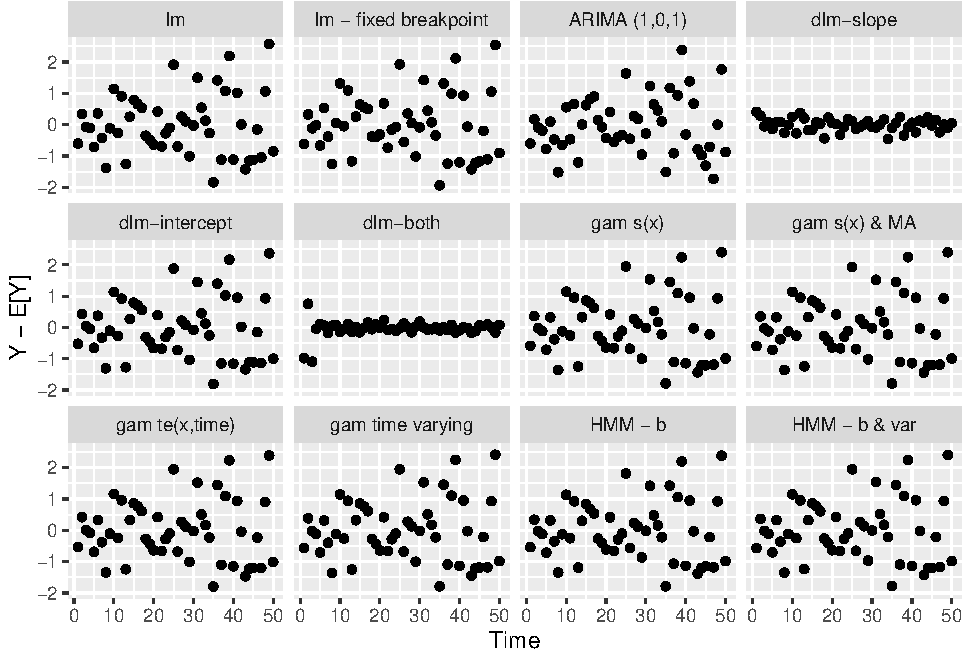
\includegraphics{univariate-time-series-examples_files/figure-latex/unnamed-chunk-7-1.pdf}
\caption{Residuals over time across models}
\end{figure}

\begin{Shaded}
\begin{Highlighting}[]
\CommentTok{# plot x versus residuals across modeling approaches}
\KeywordTok{ggplot}\NormalTok{(results, }\KeywordTok{aes}\NormalTok{(x,y}\OperatorTok{-}\NormalTok{pred)) }\OperatorTok{+}\StringTok{ }\KeywordTok{geom_point}\NormalTok{() }\OperatorTok{+}\StringTok{ }
\StringTok{  }\KeywordTok{facet_wrap}\NormalTok{(}\OperatorTok{~}\NormalTok{model) }\OperatorTok{+}\StringTok{ }\KeywordTok{xlab}\NormalTok{(}\StringTok{"Covariate (x)"}\NormalTok{) }\OperatorTok{+}\StringTok{ }\KeywordTok{ylab}\NormalTok{(}\StringTok{"Y - E[Y]"}\NormalTok{)}
\end{Highlighting}
\end{Shaded}

\begin{figure}
\centering
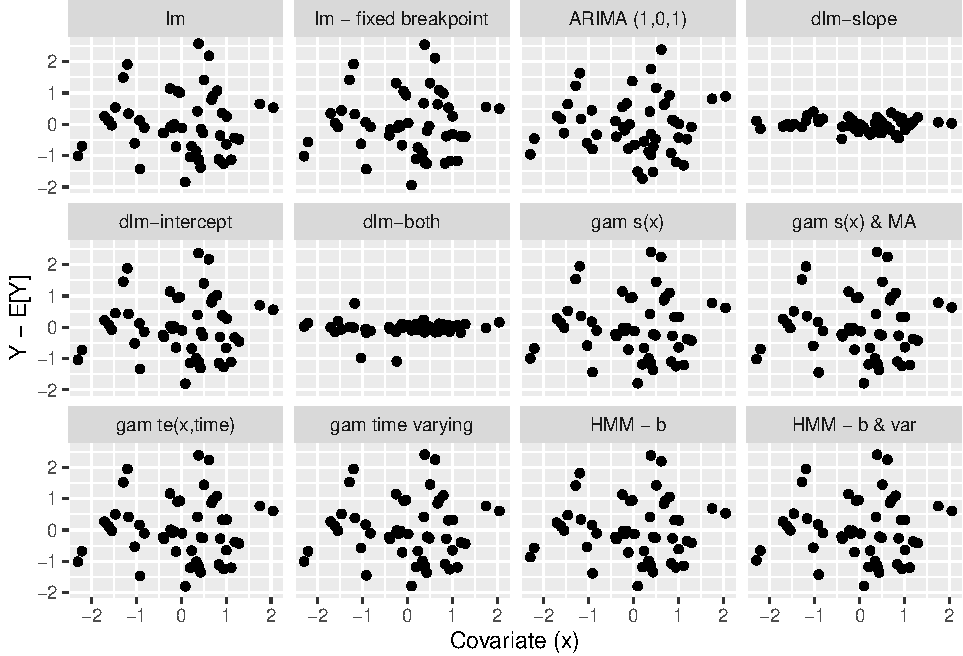
\includegraphics{univariate-time-series-examples_files/figure-latex/unnamed-chunk-8-1.pdf}
\caption{Residuals versus covariate value across models}
\end{figure}

\begin{Shaded}
\begin{Highlighting}[]
\CommentTok{# plot x versus residuals across modeling approaches}
\KeywordTok{ggplot}\NormalTok{(results, }\KeywordTok{aes}\NormalTok{(pred,y)) }\OperatorTok{+}\StringTok{ }\KeywordTok{geom_point}\NormalTok{() }\OperatorTok{+}\StringTok{ }
\StringTok{  }\KeywordTok{facet_wrap}\NormalTok{(}\OperatorTok{~}\NormalTok{model) }\OperatorTok{+}\StringTok{ }\KeywordTok{xlab}\NormalTok{(}\StringTok{"Predicted"}\NormalTok{) }\OperatorTok{+}\StringTok{ }\KeywordTok{ylab}\NormalTok{(}\StringTok{"Observed"}\NormalTok{)}
\end{Highlighting}
\end{Shaded}

\begin{figure}
\centering
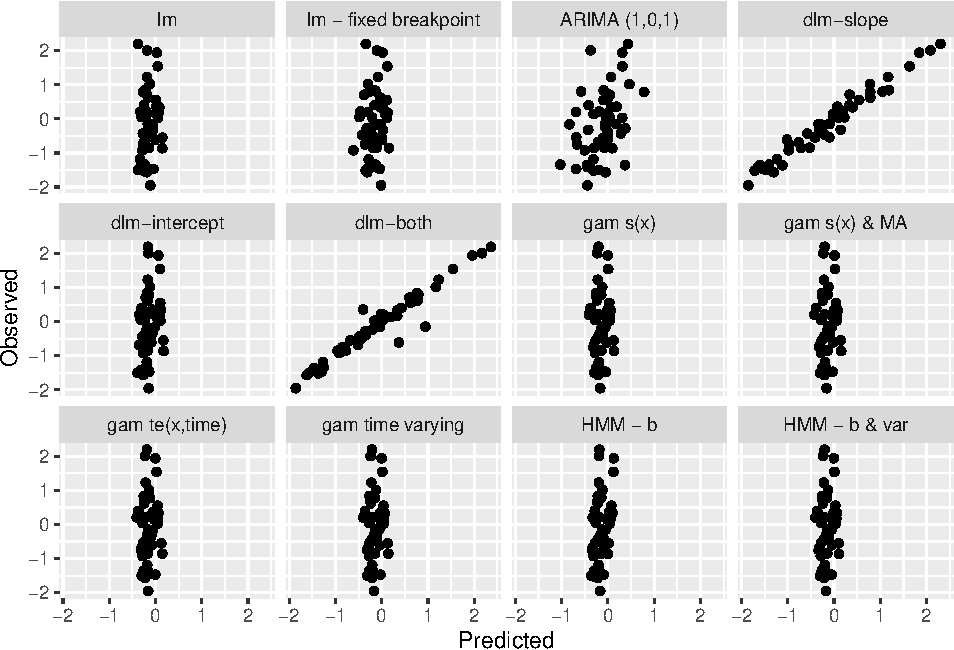
\includegraphics{univariate-time-series-examples_files/figure-latex/unnamed-chunk-9-1.pdf}
\caption{Predicted vs observed across models}
\end{figure}

\end{document}
